\section{Tính toán trục 2}
\subsection{Chọn vật liệu}
Chọn vật liệu chế tạo là thép $C_{45}$, giới hạn bền $\sigma_b =736MPa$, giới hạn chảy $\sigma_{ch} = 490MPa$.
Ứng suất uốn cho phép $[\sigma_F] = 48MPa$, ứng suất tiếp cho phép $[\tau] = 22MPa$.
\subsection{Phân tích lực trên trục}
\begin{itemize}
    \item Lực vòng bánh dẫn: $F_{t2} = F_{t1} = 2328,55N$
    \item Lực hướng tâm trên bánh bị dẫn: $F_{r2} = F_{r1} = 892,1544N$
    \item Lực dọc trục trên banh dẫn: $F_{a2} = F_{a2} = 765,588N$
    \item Lực nối trục: $F_{rk} \approx 0,2.F_{t} = 1285N$ \\
    Trong đó $F_t = \frac{2T_{II}}{D} = \frac{2.385,5}{120.10^-3} = 6425N$
\end{itemize}
\subsection{Thiết kế sơ bộ kết cấu trục}
Tính sơ bộ đường kính trục: \\
\[
    d_2 = 10\sqrt[3]{\frac{16T_2}{\pi[\tau]}} = 10\sqrt[3]{\frac{16.385,5}{\pi.22}} = 44,69(mm)
\]
$\Rightarrow$ Chọn d = 45mm theo tiêu chuẩn. \\
Khoảng cách giữa các ổ trong hộp giảm tốc bánh răng trụ một cấp: \\
\[
    l \approx l_2 + 2x + w = 85 + 2.10 + 35 = 140(mm)
\]
Trong đó: 
\begin{itemize}
    \item $l_2 = 85(mm)$ - Kết quả tính bộ truyền bánh răng
    \item $w = 35(mm) - w = 40 \div 80(mm)$ khi $T = 200 \div 400(Nm)$
    \item $x = 10(mm)$ - Khe hở giữa bánh răng và thành trong hộp giảm tốc
\end{itemize}
Khoảng cách f theo bảng 10.3 không nhỏ hơn $70 \div 105$ nên ta chọn $f = 90mm.$
\subsection{Vẽ biểu đồ momen uốn và xoắn}
Trong mặt phẳng đứng zy, phương trình cân bằng momen: $M_{A} = 0$. Suy ra:
\[
    F_{r2}.85.10^{-3} + M_{a2} + R_{BY}.140.10^{-3} = 0
\]
Trong đó $M_{a2} = \frac{F_{a2}.d_2.10^{-3}}{2} = \frac{279,367.345,27.10^{-3}}{2} = 48,23Nm$ \\
\begin{equation}
    \Leftrightarrow 892,1544.85.10^{-3} + 48,23 + R_{BY}.140.10^{-3} = 0
\end{equation}
Phương trình cân bằng lực theo trục y: \\
\[
    R_{AY}  + R_{BY} + F_{r2} = 0
\]
\begin{equation}
    \Leftrightarrow R_{AY} + R_{BY} + 892,1544 = 0
\end{equation}
Từ (3) và (4) ta giải hệ phương trình tìm được $R_{AY} = -6N$ và $R_{BY} = -886,165N$. \\
Trong mặt phẳng đứng zx, phương trình cân bằng momen: $M_{A} = 0$. Suy ra:
\[
    -F_{t2}.85.10^{-3} - F_{rk}.260.10^{-3} + R_{BX}.140.10^-3 = 0
\]
\begin{equation}
    \Leftrightarrow -2328,55.85.10^{-3} - 465,71.260.10^{-3} + R_{BX}.140.10^{-3} = 0
\end{equation}
Phương trình cân bằng lực theo trục y: \\
\[
    R_{AX} + R_{BX} - F_{t2} - F_{rk}= 0
\]
\begin{equation}
    \Leftrightarrow R_{AX} + R_{BX} - 2328,55 - 1285 = 0
\end{equation}
Từ (3) và (4) ta giải hệ phương trình tìm được $R_{AX} = 1334,9N$ và $R_{BX} = 2278,6525N$. \\
Vẽ biểu đồ momen với:
\begin{itemize}
    \item $M_{XC_1} = R_{AY}.0,085 = 0,51Nm$
    \item $M_{XC_2} = -M_{XC_1} + M_{a2} = 48,74Nm$
    \item $M_{XB} = M_{XC_2} + R_{BY}.0,085 = 0Nm$
    \item $M_{YC} = R_{AX}.0,085 = 113,4665Nm$
    \item $M_{YB} = - M_{YC} + 1285.0,085 = -4,24Nm$
\end{itemize}
Momen xoắn T2 = 385,5Nm. \\
\begin{figure}[H]
    \centering
    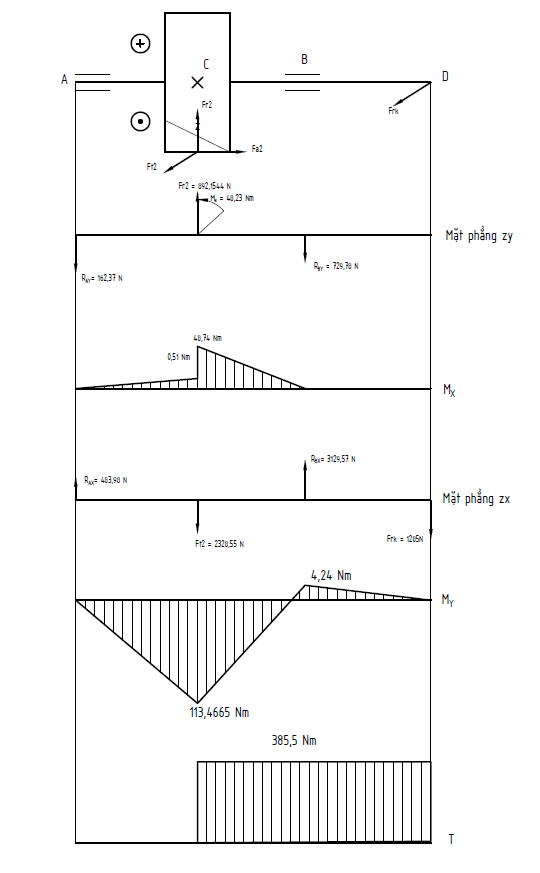
\includegraphics[width=1\textwidth]{pictures/luctruc2.png}
\end{figure}
Các biểu đồ momen cho thấy tiết diện nguy hiểm nhất tại vị trí C. \\
Momen uốn tại B:
\[
    M_B = \sqrt{M_{XC}^2 + M_{YC}^2} = \sqrt{48,74^2 + 113,4665^2} = 123,49Nm
\]
Momen xoắn tại B: $T = 385,5Nm$ \\
Momen tương đương tại C:
\[
    M_{td} = \sqrt{M_{XC}^2 + M_{YC}^2 + 0,75T^2} = \sqrt{48,74^2 + 113,4665^2 + 0,75.385,5^2} = 353,96Nm
\]
\[
d = \sqrt[3]{\frac{M_{td}.10^3}{0,1.[\sigma]}} = 41,9 mm
\]
Tại vị trí B có lắp bánh răng nên cần tăng đường kính trục thêm 5\% nên chọn d = 45mm.
\subsection{Ứng suất pháp tại tiết diện B}
Ta bỏ qua ảnh hưởng của lực dọc trục nên ứng suất pháp tại tiết diện này thay đổi theo
chu kỳ đối xứng biên độ:
\[  
    \sigma_a = \sigma_F = \frac{M_B.10^3}{W}
\]
Trục có một then, với đường kính d = 45mm, ta chọn then có chiều rộng b = 14mm, chiều cao h = 9mm, chiều sâu rãnh then trên trục t = 5,5mm, chiều sâu rãnh then trên mayơ $t_1 = 3,8 mm$. Khi đó: 
\[
    W = \frac{\pi d^3}{32} - \frac{bt(d-t)^2}{2d} = \frac{\pi 45^3}{32} - \frac{14.5,5(45-5,5)^2}{2.45} = 7516mm^3
\]
Do đó: 
\[
    \sigma_a = \frac{115,65.10^3}{7516} = 15,39MPa
\]
\subsection{Kiểm nghiệm then}
Chọn chiều dài l của then theo tiêu chuẩn l = 70mm.\\
Chọn ứng suất dập cho phép $[\sigma_d]$ = 150MPa theo bảng 16.1. \\
Chọn ứng suất cắt cho phép $[\tau_d]$ = 90MPa \\
Kiểm tra độ bền dập theo công thức:
\[
    \sigma_d = \frac{F}{t_2l_l} = \frac{2T.10^3}{t_2dl_l} = \frac{2.385,5.10^3}{3,6.45.56} = 85MPa < [\sigma_d] = 150MPa
\]
Trong đó:
\begin{itemize}
    \item $l_l = l - b = 70 - 14 = 56mm$
    \item $h = 9mm$
    \item $t_2 = 0,4h = 3,6mm$
\end{itemize}
Kiểm tra then theo độ bền cắt: 
\[
    \tau_d = \frac{T}{bl_l} = \frac{2T.10^3}{bdl_l} = \frac{2.385,5.10^3}{14.45.56} = 21,85MPa < [\tau_d] = 90MPa 
\]
$\Rightarrow$ Vậy then này đạt độ bền tính toán.
\subsection{Ứng suất xoắn}
\[
    \tau = \frac{T_2.10^3}{W_o} = \frac{385,5.10^3}{16557,5} = 23,28MPa
\]
Trong đó momen cản xoắn:
\[
    W = \frac{\pi d^3}{16} - \frac{bt(d-t)^2}{2d} = \frac{\pi 45^3}{16} - \frac{14.5,5(45-5,5)^2}{2.45} = 16557,5mm^3
\]
Khi ứng suất xoắn thay đổi theo chu kỳ mạch động: 
\[
    \tau_\alpha = \sigma_m = \frac{\sigma}{2} = \frac{23,28}{2} = 11,64MPa
\]
\subsection{Xác định hệ số an toàn}
Tại tiết diện B có sự tập trung ứng suất là rãnh then. Theo bảng 10.9 ta chọn $K_\sigma =2,05$, $K_\tau = 1,9$ với $\sigma_b = 736MPa < 800MPa$ \\
Theo bảng 10.4 với d = 45mm ta chọn $\epsilon_\sigma = 0,84$ và $\epsilon_\tau = 0.78$ \\
Hệ số $\Psi_\sigma = 0,035$ và $\Psi_\tau = 0,07$ \\ 
Với hệ số tăng bền bề mặt, chọn phương pháp phun bi nên $\beta = 1,7$. \\
Với thép C45, d =45mm chọn giới hạn mỏi của vật liệu $\sigma_{-1} = 383MPa$, $\tau_{-1} = 226MPa$. \\
Xác định hệ số an toàn tại D theo công thức:
\[
    s_\sigma = \frac{\sigma_{-1}}{K_\sigma \sigma_a / \epsilon_\sigma \beta + \Psi_\sigma \sigma_m} = \frac{383}{2,05.15,39/0,84.1,7 + 0,035.0} = 17,335
\]
\[
    s_\tau = \frac{\tau_{-1}}{K_\tau \tau_a / \epsilon_\tau \beta + \Psi_\tau \tau_m} = \frac{226}{2,05.11,64/0,78.1,7 + 0,07.11,64} = 12,015
\]
Hệ số an toàn:
\[
    s = \frac{s_\sigma s_\tau}{\sqrt{s_\sigma^2 + s_\tau^2}} = \frac{17,335.12,015}{\sqrt{17,335^2 + 12,015^2}} = 9,875 > [s] = 1,5
\]
Do đó điều kiện bền mỏi của trục tại tiết diện B được thỏa.
\cleardoublepage